\documentclass[11pt]{article}
\usepackage[UTF8]{ctex}
\usepackage[a4paper]{geometry}
\geometry{left=2.0cm,right=2.0cm,top=2.5cm,bottom=2.5cm}

\usepackage{caption}
\usepackage{paralist}
\usepackage{enumitem}
\setenumerate[1]{itemsep=0pt,partopsep=0pt,parsep=0pt,topsep=0pt}
\setitemize[1]{itemsep=0pt,partopsep=0pt,parsep=0pt,topsep=0pt}
\usepackage{comment}
\usepackage{booktabs}
\usepackage{graphicx}
\usepackage{float}
\usepackage{diagbox}
\usepackage{amsmath,amsfonts,graphicx,amssymb,bm,amsthm}
\usepackage{algorithm,algorithmicx}
% \usepackage[ruled, linesnumbered]{algorithm2e}
% \usepackage[linesnumbered]{algorithm2e}
\usepackage[noend]{algpseudocode}
\usepackage{fancyhdr}
\usepackage{tikz}
\usepackage{graphicx}
\usetikzlibrary{arrows,automata,positioning}
\usepackage{hyperref}
\usepackage{extarrows}
% 这是一些字体选项
\usepackage{helvet}
% \usepackage{mathpazo}
\usepackage{fontspec}
% \setmainfont{Times New Roman}
% \setmainfont{Comic Sans MS} % 比较fancy的字体
% \setmainfont{Avenir}
% \setmainfont{Palatino}

\setlength{\headheight}{14pt}
\setlength{\parindent}{0 in}
\setlength{\parskip}{0.5 em}


\newtheorem{theorem}{Theorem}
\newtheorem{lemma}[theorem]{Lemma}
\newtheorem{proposition}[theorem]{Proposition}
\newtheorem{claim}[theorem]{Claim}
\newtheorem{corollary}[theorem]{Corollary}
\newtheorem{definition}[theorem]{Definition}
\newtheorem*{definition*}{Definition}

\newenvironment{problem}[2][Problem]{\begin{trivlist}
\item[\hskip \labelsep{\bfseries#1}\hskip\labelsep{\bfseries#2.}]}{\hfill$\blacktriangleleft$\end{trivlist}}
\newenvironment{answer}[1][Answer]{\begin{trivlist}
\item[\hskip \labelsep{\bfseries\itshape#1.}\hskip \labelsep]}{\hfill$\lhd$\end{trivlist}}

\newcommand\E{\mathbb{E}}
\newcommand\per{\mathrm{per}}
\renewcommand{\algorithmicrequire}{\textbf{Input:}}
\renewcommand{\algorithmicensure}{\textbf{Output:}}
\algrenewcommand{\algorithmiccomment}[1]{\hfill $//$ #1}
% chktex-file 44
% \renewcommand{\familydefault}{\sfdefault}

\RequirePackage{algorithm}

\makeatletter
\newenvironment{breakablealgorithm}
  {% \begin{breakablealgorithm}
    \begin{center}
      \refstepcounter{algorithm}% New algorithm
      \hrule height.8pt depth0pt \kern2pt% \@fs@pre for \@fs@ruled
      \parskip 0pt
      \renewcommand{\caption}[2][\relax]{% Make a new \caption
        {\raggedright\textbf{\fname@algorithm~\thealgorithm} ##2\par}%
        \ifx\relax##1\relax % #1 is \relax
          \addcontentsline{loa}{algorithm}{\protect\numberline{\thealgorithm}##2}%
        \else % #1 is not \relax
          \addcontentsline{loa}{algorithm}{\protect\numberline{\thealgorithm}##1}%
        \fi
        \kern2pt\hrule\kern2pt
     }
  }
  {% \end{breakablealgorithm}
     \kern2pt\hrule\relax% \@fs@post for \@fs@ruled
   \end{center}
  }
\makeatother

% set for automata
\tikzset{>=stealth',shorten >=1pt,auto,node distance=2cm, % Increase node distance to 4cm
                    thick,main node/.style={circle,draw,font=\sffamily\Large\bfseries}}


\title{Homework \#5}
\usetikzlibrary{positioning}

\begin{document}
\captionsetup[figure]{labelfont={bf},name={Fig.},labelsep=period}
\kaishu

\pagestyle{fancy}
\lhead{\CJKfamily{zhkai} Peking University}
\chead{}
\rhead{\CJKfamily{zhkai} Algorithm Design and Analysis (Honor Track)}

\begin{center}
    {\LARGE \bf Homework 5}\\
    {Name: 方嘉聪\ \  ID: 2200017849}            % Write down your name and ID here.
\end{center}

\begin{problem}{1. (Textbook 5.9)}
    \songti
    设有$n$项任务由$k$个可并行操作的机器完成, 完成任务$i$所需要的时间为$t_i$.求一个最佳任务分配方案, 使得完成时间(即从时刻0计时, 到最后一台机器停止的时间)达到最短. 
    \label{problem_1}
\end{problem}
\begin{answer}
设$n$个任务的编号为$1,2,\cdots,n$, $k$台机器的编号为$1,2,\cdots,k$. 使用深度优先遍历, 根节点分支出$k$条边, 分别表示任务1分配给机器1, 2, $\cdots$, $k$. 递归地, 对于每个节点, 分支出$k$条边, 表示任务2分配给机器1, 2, $\cdots$, $k$. 以此类推, 直到任务$n$分配给机器1, 2, $\cdots$, $k$, 由此可以得到$k^n$个分配方案.
\\用$<i_1, i_2, \cdots, i_n>(\forall j \in \{1,2, \cdots, n\}, ~ 1\le i_j\le k)$表示任务$1, 2, \cdots, n$分配到了机器$i_1, i_2, \cdots, i_n$.对于每一个分配方案, 对每个机器$j$会得到一个任务序列$w_1, w_2, \cdots, w_{u_j}$, 计算$u_j$个任务完成的总时间, 即为机器$j$的完成时间. 从中选取最大的完成时间, 即为这个分配方案的完成时间. 时间复杂度为$O(n k^n)$.
\\从所有的分配方案中选取完成时间最短的一个, 即为最优的任务分配方案. 时间复杂度为$O(k^n)$.故总的时间复杂度为$O(n k^n)$.
\end{answer}

\begin{problem}{2. (Textbook 5.10)}
    \songti
在\textbf{Problem 1}中, 假设每个任务有个完成期限$B_i$, 以及超出期限的罚款数$f_i$. 试求一个最佳任务分配方案, 使得罚款总和最小.
\end{problem}
\begin{answer}
类似\textbf{Problem 1}得到任务分配方案$<i_1, i_2, \cdots, i_n>$(时间复杂度$O(n \cdot k^n)$). 对于每个任务分配方案, 设机器$j$分到的任务为$w_1, w_2, \cdots, w_{u_j}$. 遍历任务序列的不同排列, 计算各个顺序下的罚款总和, 选取最小的一个排列(解空间是一个排列树, 按照深度优先遍历), 时间复杂度为$O(n \cdot n! \cdot k^n)$. 最后从$k^n$个方案中选取总罚款数最小的任务分配方案, 时间复杂度为$O(k^n)$.故整个问题的时间复杂度为$O(n \cdot n! \cdot k^n)$.
\end{answer}

\begin{problem}{3. (Minimizing Kendall tau distance)}
    Given $m$ rank lists denoted as $P_1, P_2, \dots, P_m$, each of which is a permutation of integers from $1$ to $n$. We want to find an aggregation rank list $S$ which is also a permutation of integers from $1$ to $n$, and minimizes the \textit{Kendall tau distance} between $S$ and $P_1, P_2, \dots, P_m$.
    \\Kendall tau distance is defined as:
    \begin{align*}
        K(S;P_1,P_2,P_3,\dots,P_m) = \sum_{k=1}^{m} |\left\{(i,j)\ |\ \mathrm{rank}(i,P_k)<\mathrm{rank}(j,P_k)\ \mathrm{and}\ \mathrm{rank}(i,S) > \mathrm{rank}(j,S)\right\}| 
    \end{align*}
    where $\mathrm{rank}(i,P)$ represents the rank of $i$ in permutation $P$.
    Please use the \textbf{branch-and-bound} method to solve this problem and provide \textbf{complexity analysis}.
\end{problem}
\begin{answer}
注意到$K(S;P_1) = |\left\{(i,j)\ |\ \mathrm{rank}(i,P_1)<\mathrm{rank}(j,P_1)\ \mathrm{and}\ \mathrm{rank}(i,S) > \mathrm{rank}(j,S)\right\}| $等价于计算以$P_1$为参照$S$的逆序对数.那么使用归并排序的思想, 可以在$O(n\log n)$的时间内计算出$K(S;P_1)$.
\\按照字典顺序生成$1, 2, \cdots, n$的一个排列的树, 用深度优先搜索遍历这个树,时间复杂度为$O(n!)$. 每次遍历到叶子节点时, 计算$K(S;P_1, P_2, \cdots, P_m)$(时间复杂度为$O(m n\log n)$), 并更新最小值. 总的时间复杂度为$O(n! m n \log n)$.
\\下面叙述如何通过分支限界技术来进行剪枝, 设$A_{t,k} = <i_1, i_2, \cdots, i_k>$为当前的排列($t$属于一个表示所有$n!$排列的指标集), $L$为当前的最小距离(初始化为$\infty$). 设代价函数(估计$A_{t,k}$的Kendall tau distance下界)为$F(A_{t,k})$, $dis(A_{t,k})$表示目前得到的Kendall tau distance. 则有以下剪枝策略:
\\1. 若$dis(A_{t,k}) + F(A_{t,k})\ge L$, 则剪枝.
\\2. 若$K(S_t;P_1, P_2, \cdots, P_m) < L $, 则更新$L$.

$F(A_{t,k})$的定义为: 
\\计算$i_1, i_2, \cdots, i_k$出现在$P_j(\forall j \in \{1,2,\cdots, m\})$的后$n-k$位的次数, 记为$C_{j,t,k}$,实现上可以直接扫描一遍, 计算一个$C_{j,t,k}$的时间复杂度为$O(k(n-k))$. 计算所有的$C_{j,t,k}$, 总的时间复杂度会增加$O(n!\cdot m\cdot n^3 )$,
\\令$F(A_{t,k}) = \sum_{j=1}^{m} C_{j,t,k}^2$.这是由于在最理想的情况下, 假设可以做到$S$的后$n-k$对于所有的$P_j$都没有逆序对, 那么只要考虑$S$的后$n-k$个元素与$P_j$的后$k$个元素的逆序对数.对每个$P_j$, $C_{j,t,k}^2$即为一个下界.故这样定义的$F(A_{t,k})$是一个合适的代价函数.
\\ 故最终总的时间复杂度为$O(n!\cdot m\cdot n^3)$.在实际应用中可能对不同情况再具体评估一下剪枝的效果.

\end{answer}

\begin{problem}{4. (Circuit Routing)}
    As shown in Figure \ref{fig_routing}, the printed circuit board (PCB) divides the wiring area into an $m\times n$ grid array. We want to determine the shortest routing scheme connecting the grid \textbf{a} to the grid \textbf{b}. To avoid crossing lines, the grid with already routed wires has been marked as blocked (as shown in \textbf{1} in Figure \ref{fig_routing}), and other lines are not allowed to pass through the blocked grid. When routing, the circuit wires can only be routed in a straight line or at a right angle. Please use the \textbf{branch-and-bound} method to solve this problem, explain the specific process, and analyze the \textbf{time complexity} of the algorithm (worst case).
    \begin{figure}[H]
        \centering
        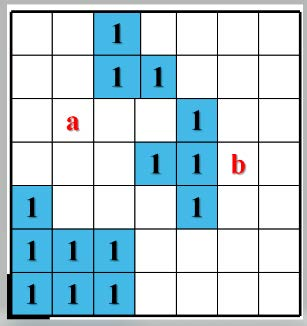
\includegraphics[width=0.3\textwidth]{images/routing.jpg}
        \caption{PCB routing example}
        \label{fig_routing}
    \end{figure}
\end{problem}
\begin{answer}
    使用优先队列实现的广度优先搜索(回溯,每个节点只访问一次), 从\textbf{a}开始, 先将其周围的合法节点加入优先队列中, 优先队列按照代价(记为$f(a)$)从小到大排序. 每次取出代价最小的节点进行扩展, 直到取出的节点为终点或者优先队列为空. 时间复杂度为$O(mn\log(mn))$.
    
    进一步剪枝优化, 给每个格点一个坐标$(i,j).$采用$A^*$搜索, 设节点$A$的代价$f(A) = g(A) + h(A)$, 其中$g(A)$表示目前已经走过的路径长度, $h(A)$为启发函数. 这里取$h(A)$为$A$到终点(记为$B$)的曼哈顿距离$|x_a - x_b| + |y_a - y_b|$, 显然$h(A)$是$A$到$B$的最短距离的一个下界, 故$A^*$搜索的结果一定是最优解, 时间复杂度为$O(mn\log(mn))$.
\end{answer}
\end{document}